\documentclass[12pt,a4paper]{report}
\usepackage[T2A]{fontenc}
\usepackage[utf8]{inputenc}
\usepackage[russian]{babel}
\usepackage{graphicx, setspace, amsmath}


\usepackage[
top = 1.25cm,
bottom = 2.0cm]{geometry}

\begin{document}
\begin{titlepage}
    \centering
    % HEADER
    {
        \scshape
        Федеральное государственное автономное образовательное учреждение высшего образования
        \par
        \textbf{«Научно-образовательная корпорация ИТМО»}
        \par
        \vspace*{1cm}
        Факультет Программной Инженерии и Компьютерной Техники
        \par
    }
    % LOGO
    \vspace*{0.6cm}
    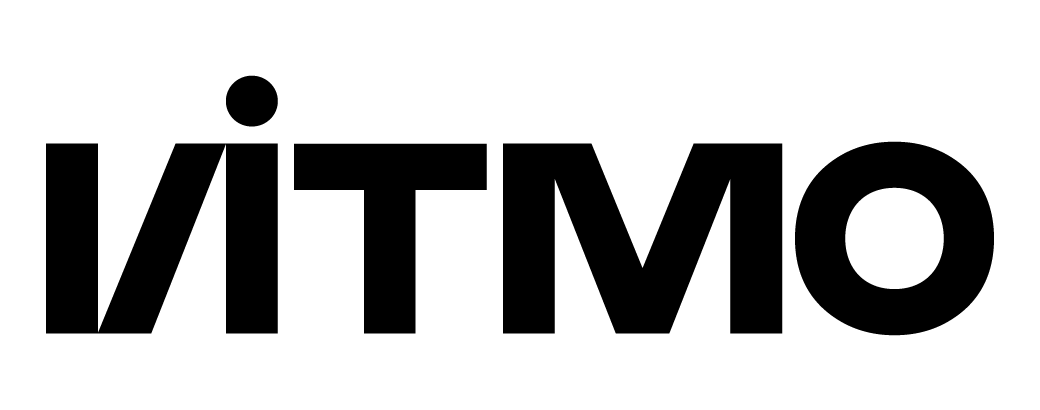
\includegraphics[width=\textwidth]{logo.png}
    % LAB INFO
    {
        \Large
        \textbf{Домашняя работа по представлению чисел в ЭВМ №7}
        \par
        \normalsize
        \vspace*{0.75cm}
        \textbf{Вариант 39}
        \par
    }
    \vfill
    % СREDITS
    \hfill\begin{minipage}{\dimexpr\textwidth-7.8cm}
        \textbf{Выполнил:}\par
        Степанов Арсений Алексеевич\par
        \vspace*{0.15cm}
        \textbf{Группа:}\par
        P3109\par
        \vspace*{0.15cm}
        \textbf{Преподаватель:}\par
        Поляков Владимир Иванович\par
    \end{minipage}
    \vfill
    Санкт-Петербург, \the\year{}г.
\end{titlepage}
\onehalfspacing
\section*{Значения чисел для данного варианта}
$A=3.9_{10}\approx3.E666_{16}=11.1110011001100110_2$\\
$A_{F1}=0.1000001.0011\;1110\;0110$\\
$A_{F2}=0.10000010.1111\;0011\;001$\\
$B=0.44_{10}\approx0.70A3_{16}=0.01110000101000111101$\\
$B_{F1}=0.1000000.0111\;0000\;1010$\\
$B_{F2}=0.01111111.1100\;0010\;100$
\section*{Задание №1}
$X_C=X_A+X_B-2^6=65_{10}=1000001_2$\\
$C_{sign}=0$\\
\hfill\break
\begin{tabular}{|c|c|c|c|}
\hline
СЧП(ст.р.) & СЧП(мл.р.) & К & Д\\
\hline
$000000000000000$ & $0111000010\underline{10}$ & $0$ & - \\ 
\hline
    $
        \begin{array}{r}
        +
        \begin{array}{r}
        000000000000000\\
        000011111001100
        \end{array}\\
        \hline
        \begin{array}{r}
        000011111001100
        \end{array}\\
        \end{array}
    $ & & $0$ & +2A\\
\hline
$000000111110011$ & $00|01110000\underline{10}$ & $0$ & $\rightarrow$2СЧП\\
\hline
    $
        \begin{array}{r}
        +
        \begin{array}{r}
        000\overset{\small{1}}{0}\overset{\small{1}}{0}\overset{\small{1}}{0}\overset{\small{1}}{1}\overset{\small{1}}{1}1110011\\
        000011111001100
        \end{array}\\
        \hline
        \begin{array}{r}
        000100110111111
        \end{array}\\
        \end{array}
    $ & & $0$ & +2A\\
\hline
$000001001101111$ & $1100|011100\underline{00}$ & $0$ & $\rightarrow$2СЧП\\
\hline
$000000010011011$ & $111100|0111\underline{00}$ & $0$ & $\rightarrow$2СЧП\\
\hline
$000000000100110$ & $11111100|01\underline{11}$ & $0$ & $\rightarrow$2СЧП\\
\hline
    $
        \begin{array}{r}
        -
        \begin{array}{r}
        \overset{\small{1}}{\phantom{0}}\overset{\small{1}}{0}\overset{\small{1}}{0}\overset{\small{1}}{0}\overset{\small{1}}{0}\overset{\small{1}}{0}\overset{\small{1}}{0}\overset{\small{1}}{0}\overset{\small{1}}{0}0100110\\
        000001111100110
        \end{array}\\
        \hline
        \begin{array}{r}
        111110001000000
        \end{array}\\
        \end{array}
    $ & & $1$ & -A\\
\hline
$111111100010000$ & $0011111100|\underline{01}$ & $1$ & $\rightarrow$2СЧП\\
\hline
    $
        \begin{array}{r}
        +
        \begin{array}{r}
        \overset{\small{1}}{\phantom{0}}\overset{\small{1}}{1}\overset{\small{1}}{1}\overset{\small{1}}{1}\overset{\small{1}}{1}\overset{\small{1}}{1}\overset{\small{1}}{1}100010000\\
        000011111001100
        \end{array}\\
        \hline
        \begin{array}{r}
        000011011011100
        \end{array}\\
        \end{array}
    $ & & $0$ & +2A\\
\hline
$000000110110111$ & $000011111100$ & $0$ & $\rightarrow$2СЧП\\
\hline
\end{tabular}\\
\hfill\break
$M_A=0001\;1011\;0111_2$\\
$C=0.1000001.0001\;1011\;0111_{F1}$\\
$C^*=0.0001\;1011\;0111_2\cdot16^1=1.1011\;0111_2=1.71484375_{10}$\\
$C_T=3.9\cdot0.44=1.716$\\
$\delta C=|\dfrac{C_T-C^*}{C_T}|\cdot100\%\approx0.0673805\%$
\section*{Задание №2}
$X_C=X_A+X_B-2^7=129_{10}=10000001_2$\\
$C_{sign}=0$\\
\hfill\break
\begin{tabular}{|c|c|c|c|}
    \hline
    СЧП(ст.р.) & СЧП(мл.р.) & К & Д\\
    \hline
    $00000000000000000$ & $01110000\underline{1010}$ & $0$ & -\\
    \hline
        $
            \begin{array}{r}
            +
            \begin{array}{r}
            00000000000000000\\
            00001111100110000
            \end{array}\\
            \hline
            \begin{array}{r}
            00001111100110000
            \end{array}\\
            \end{array}
        $ & & $0$ & +8A\\
    \hline
        $
            \begin{array}{r}
            +
            \begin{array}{r}
            000\overset{\small{1}}{0}\overset{\small{1}}{1}\overset{\small{1}}{1}\overset{\small{1}}{1}\overset{\small{1}}{1}100110000\\
            00000011111001100
            \end{array}\\
            \hline
            \begin{array}{r}
            00010011011111100
            \end{array}\\
            \end{array}
        $ & & $0$ & +2A\\
    \hline
    $00000001001101111$ & $1100|0111\underline{0000}$ & $0$ & $\rightarrow$4СЧП\\
%    \hline
%        $
%            \begin{array}{r}
%            +
%            \begin{array}{r}
%            00000001001101111\\
%            00000000000000000
%            \end{array}\\
%            \hline
%            \begin{array}{r}
%            00000001001101111
%            \end{array}\\
%            \end{array}
%        $ & & $0$\\
%    \hline
%        $
%            \begin{array}{r}
%            +
%            \begin{array}{r}
%            00000001001101111\\
%            00000000000000000
%            \end{array}\\
%            \hline
%            \begin{array}{r}
%            00000001001101111
%            \end{array}\\
%            \end{array}
%        $ & & $0$\\
    \hline
    $00000000000100110$ & $11111100|\underline{0111}$ & $0$ & $\rightarrow$4СЧП\\
    \hline
        $
            \begin{array}{r}
            +
            \begin{array}{r}
            0000000000\overset{\small{1}}{0}100110\\
            00001111100110000
            \end{array}\\
            \hline
            \begin{array}{r}
            00001111101010110
            \end{array}\\
            \end{array}
        $ & & $0$ & +8A\\
    \hline
        $
            \begin{array}{r}
            -
            \begin{array}{r}
            000011\overset{\small{1}}{1}\overset{\small{1}}{1}\overset{\small{1}}{1}\overset{\small{1}}{0}\overset{\small{1}}{1}010110\\
            00000001111100110
            \end{array}\\
            \hline
            \begin{array}{r}
            00001101101110000
            \end{array}\\
            \end{array}
        $ & & $0$ & -A\\
    \hline
    $00000000110110111$ & $000011111100$ & $0$ & $\rightarrow$4СЧП\\
    \hline
    $00000110110111000$ & $011111100000$ & $0$ & $\leftarrow$3СЧП\\
    \hline
    \end{tabular}\\
    \hfill\break
    $M_A=1011\;0111\;000_2$\\
    $C=0.10000001.1011\;0111\;000_{F1}$\\
    $C^*=0.1101\;1011\;1000_2\cdot2^1=1.1011\;0111_2=1.71484375_{10}$\\
    $C_T=3.9\cdot0.44=1.716$\\
    $\delta C=|\dfrac{C_T-C^*}{C_T}|\cdot100\%\approx0.0673805\%$\\
\end{document}